\usepackage{booktabs}

% bibliography settings
% 适用于中文文章的 GBT-7714 参考文献格式
% https://ctan.org/pkg/gbt7714?lang=en
% https://github.com/zepinglee/gbt7714-bibtex-style
\usepackage{gbt7714}
\bibliographystyle{gbt7714-numerical} % 参考文献样式
% 配置字体、颜色、框（tcolorbox）样式

% 配置中文主字体：指定fonts目录下的Fandol字体
\usepackage{fontspec}

% 中文主字体：Fandol 宋体（含粗体、斜体配置）
\setCJKmainfont[
  Path       = fonts/,    % 字体文件所在相对路径（确保路径正确）
  Extension  = .otf,      % 字体文件扩展名
  BoldFont   = FandolHei-Regular,  % 粗体字体名
  ItalicFont = FandolKai-Regular   % 斜体（楷体）字体名
]{FandolSong-Regular}

% 中文无衬线字体：Fandol 黑体
\setCJKsansfont[
  Path       = fonts/,
  Extension  = .otf,
  BoldFont   = FandolHei-Bold
]{FandolHei-Regular}

% 中文等宽字体：Fandol 仿宋
\setCJKmonofont[
  Path       = fonts/,
  Extension  = .otf
]{FandolFang-Regular}

% 中文字族（同样修正参数格式）
\setCJKfamilyfont{zhsong}[
  Path       = fonts/,
  Extension  = .otf,
  BoldFont   = FandolHei-Regular
]{FandolSong-Regular}

\setCJKfamilyfont{zhhei}[
  Path       = fonts/,
  Extension  = .otf,
  BoldFont   = FandolHei-Regular
]{FandolHei-Regular}

\setCJKfamilyfont{zhfs}[
  Path       = fonts/,
  Extension  = .otf
]{FandolFang-Regular}

\setCJKfamilyfont{zhkai}[
  Path       = fonts/,
  Extension  = .otf
]{FandolKai-Regular}

% 字体命令
\renewcommand{\songti}{\CJKfamily{zhsong}}
\renewcommand{\heiti}{\CJKfamily{zhhei}}
\renewcommand{\fangsong}{\CJKfamily{zhfs}}
\renewcommand{\kaishu}{\CJKfamily{zhkai}}

% color settings
\definecolor{shallow-frame}{RGB}{211, 211, 211}
\definecolor{shallow-background}{RGB}{240, 240, 240}
\definecolor{warm-background}{RGB}{239, 239, 221}
\definecolor{blue-background}{RGB}{214, 220, 229}
\definecolor{deepblue-background}{RGB}{141, 170, 212}
\definecolor{darkgray-background}{RGB}{217, 217, 217}
\definecolor{mydarkgray}{RGB}{76, 76, 76}

\usepackage[most]{tcolorbox}

% tcolorbox
\newtcolorbox{mybox}[1]{
  colback=darkgray-background!40,
  coltitle=black,
  colframe=darkgray-background,
  colbacktitle=darkgray-background!60,
  fonttitle=\heiti,
  title={#1}
}

\newtcolorbox{mynotice}{
  colback=darkgray-background!40,
  colframe=darkgray-background,
}

\newtcolorbox{mynote}[1]{
  title={#1},
  coltitle=black,
  fonttitle=\heiti,
  colback=white,
  colframe=darkgray-background!60,
} % 页面设计
\usepackage[
    acronym,
    style=index,
    nonumberlist=false,
    counter=page,
    hyperfirst=false,
    xindy={language=simplified-chinese},
    hyperfirst=true,
    ]{glossaries}

\makeglossaries

% ===== 以下为模板使用手册相关术语 =====
\newglossaryentry{cursor}{
    name={Cursor},
    first={Cursor},
    description={以 AI 辅助编程为核心的编辑器环境，可用于本模板的本地写作与编译管理。},
    sort={cursor}
}

\newglossaryentry{vscode}{
    name={VS Code},
    first={VS Code},
    description={常用代码编辑器，可配合 LaTeX 插件完成论文模板编辑与构建。},
    sort={vs code}
}

\newglossaryentry{overleaf}{
    name={Overleaf},
    first={Overleaf},
    description={在线 LaTeX 编辑平台，适合轻量协作与预览，但大型工程可能出现编译耗时较长。},
    sort={overleaf}
}

\newglossaryentry{texlive}{
    name={TeX Live},
    first={TeX Live},
    description={主流 TeX 发行版之一，提供论文模板编译所需工具链。},
    sort={tex live}
}

\newglossaryentry{miktex}{
    name={MiKTeX},
    first={MiKTeX},
    description={常用 TeX 发行版之一，可作为本模板本地编译环境。},
    sort={miktex}
}

\newglossaryentry{xelatex}{
    name={XeLaTeX},
    first={XeLaTeX},
    description={支持 Unicode 与系统字体的 LaTeX 引擎，适合中文论文排版。},
    sort={xelatex}
}

\newglossaryentry{latexworkshop}{
    name={LaTeX Workshop},
    first={LaTeX Workshop},
    description={VS Code/Cursor 常用 LaTeX 扩展，支持构建链、日志定位与 PDF 预览。},
    sort={latex workshop}
}

\newglossaryentry{bibtex-tool}{
    name={BibTeX},
    first={BibTeX},
    description={用于处理参考文献数据库并生成文献列表的工具。},
    sort={bibtex tool}
}

\newglossaryentry{tikz}{
    name={TikZ},
    first={TikZ},
    description={LaTeX 绘图库，可直接在文档中定义流程图、结构图等矢量图形。},
    sort={tikz}
}

\newglossaryentry{pgfplots}{
    name={PGFPlots},
    first={PGFPlots},
    description={基于 TikZ 的绘图包，常用于函数图和实验结果可视化。},
    sort={pgfplots}
}

\newglossaryentry{cleverefpkg}{
    name={cleveref},
    first={cleveref},
    description={交叉引用增强宏包，可自动补充图、表、公式和章节等引用前缀。},
    sort={cleveref package}
}

\newglossaryentry{glossariespkg}{
    name={glossaries},
    first={glossaries},
    description={术语表与缩略语管理宏包，可统一术语首次出现与索引输出。},
    sort={glossaries package}
} % glossaries 包，用于导入术语与符号
% 配置绘图（tikz 与 pgfplots）样式
\usepackage{tikz}

\usetikzlibrary{
  shapes.geometric,
  arrows,
  positioning,
  fit,
  calc,
  shapes,
  backgrounds,
  matrix,
  pgfplots.groupplots
}
\usepackage{pgfplots}
\pgfplotsset{compat=1.18}
\usepackage{tikz-3dplot}
\tdplotsetmaincoords{70}{120}

\tikzset{
  block/.style={
      rectangle,
      rounded corners,
      minimum width=2.5cm,
      minimum height=1cm,
      text centered,
      draw=black,
      line width=1pt,
      fill=deepblue-background
    },
  circle/.style={
      draw=darkgray,
      line width=1pt,
      fill=darkgray-background,
      opacity=0.2
    },
  line/.style={thick, -, color=black},
  arrow/.style={thick, ->, >=stealth, color=black}
}

\pgfdeclarelayer{bg1}
\pgfdeclarelayer{bg2}
\pgfdeclarelayer{bg3}
\pgfdeclarelayer{fg1}
\pgfdeclarelayer{fg2}
\pgfdeclarelayer{fg3}
\pgfsetlayers{bg1,bg2,bg3,main,fg1,fg2,fg3}

 % 绘图
\usepackage{float}
\usepackage{algorithm}
\usepackage{algorithmic}

\usepackage[most]{tcolorbox}

\newtcolorbox{mybox}[1]{
  colback=darkgray-background!40,
  coltitle=black,
  colframe=darkgray-background,
  colbacktitle=darkgray-background!60,
  fonttitle=\heiti,
  title={#1}
}

\newtcolorbox{mynotice}{
  colback=darkgray-background!40,
  colframe=darkgray-background,
}

\newcommand{\x}{\boldsymbol{x}}
\newcommand{\z}{\boldsymbol{z}}
\newcommand{\xa}{\boldsymbol{x}^{adv}}
\newcommand{\w}{\mathbf{w}}
\newcommand{\p}{\boldsymbol{p}}
\newcommand{\q}{\boldsymbol{q}}
\renewcommand{\v}{\boldsymbol{v}}
\renewcommand{\u}{\boldsymbol{u}}
\renewcommand{\o}{\boldsymbol{o}}
\renewcommand{\b}{\boldsymbol{b}}
\newcommand{\h}{\boldsymbol{h}}
\renewcommand{\H}{\mathcal{H}}

\newcommand{\dpr}{d^{\prime}}

\newcommand{\A}{\boldsymbol{A}}
\newcommand{\M}{\boldsymbol{M}}
\newcommand{\X}{\boldsymbol{X}}
\newcommand{\W}{\boldsymbol{W}}

\newcommand{\bmu}{\boldsymbol{\mu}}

\newcommand{\calX}{\mathcal{X}}
\newcommand{\calR}{\mathcal{R}}
\newcommand{\calH}{\mathcal{H}}
\newcommand{\calD}{\mathcal{D}}
\newcommand{\D}{\mathcal{D}}
\newcommand{\calN}{\mathcal{N}}
\newcommand{\calF}{\mathcal{F}}

\newcommand{\R}{\mathbb{R}}

\DeclareMathOperator{\reg}{\text{reg}}
\DeclareMathOperator{\relu}{\text{ReLU}}
\DeclareMathOperator{\softmax}{\text{softmax}}
\DeclareMathOperator{\argmax}{\text{argmax}}
\DeclareMathOperator{\argmin}{\text{argmin}}

% NC
\newcommand{\iter}[1]{\{#1\}}
\newcommand{\bbeta}{\boldsymbol{\beta}}
\newcommand{\Radv}{R_{\rm{adv}}}
\newcommand{\Rstd}{R_{\rm{std}}}
\newcommand{\1}{\boldsymbol{1}}
\newcommand{\0}{\boldsymbol{0}}
\newcommand{\I}{\boldsymbol{I}}
\renewcommand{\o}{\boldsymbol{o}}
\DeclareMathOperator\srelu{sReLU}

% RBAD
\usepackage{bm}
\usepackage{subcaption}
\newcommand{\V}{\mbox{Vol}}
\newcommand{\ip}[1]{\left\langle #1 \right\rangle}
\newcommand{\ipsmall}[1]{\langle #1 \rangle}
\newcommand{\qm}[1]{``#1''}
\renewcommand{\P}{\boldsymbol{P}}
\newcommand{\risk}{\mathcal{R}}
\newcommand{\Z}{\mathcal{Z}}
\newcommand{\N}{\mathcal{N}}
\newcommand{\smost}{\tilde{\S}}
\newcommand{\sless}{\S_{less}}
\newcommand{\snot}{\S_{not}}
\newcommand{\smostbound}{t \sigma_0 c_1 f_h}
\newcommand{\slessbound}{t \sigma_0 f_r}
\newcommand{\wbound}{t \sigma_0 f_h}
\newcommand{\cone}{\hat{\S}}
\newcommand{\MM}{\mathbf{M}}
\newcommand{\relup}[1]{ \sigma^{\prime} \left( #1 \right)} % ReLU
\newcommand{\E}{\mathbb{E}}

\renewcommand{\paragraph}[1]{\vspace{0.5em}\noindent{\heiti{#1}}\hspace{0.5em}} % 快捷键
\usepackage{cleveref}
\refname{equation}{式}{式}
\refname{figure}{图}{图}
\refname{table}{表}{表}
\refname{page}{页}{页}
\refname{chapter}{章}{章}
\refname{section}{节}{节}
\refname{appendix}{附录}{附录}
\refname{theorem}{定理}{定理}
\refname{lemma}{引理}{引理}
\refname{corollary}{推论}{推论}
\refname{proposition}{命题}{命题}
\refname{definition}{定义}{定义}
\refname{example}{例}{例}
\refname{algorithm}{算法}{算法}
\refname{listing}{列表}{列表}
\refname{line}{行}{行}

\refformat{chapter}{#2第#1章#3}
\refformat{section}{#2第#1节#3}
\refformat{subsection}{#2第#1节#3}
\refformat{subsubsection}{#2第#1节#3}

\refrangeformat{chapter}{#3第#1章#4至#5第#2章#6}
\refrangeformat{section}{#3第#1节#4至#5第#2节#6}
\refrangeformat{subsection}{#3第#1节#4至#5第#2节#6}
\refrangeformat{subsubsection}{#3第#1节#4至#5第#2节#6}

\refmultiformat{chapter}{#2第#1章#3}{和#2第#1章#3}{，#2第#1章#3}{和#2第#1章#3}
\refmultiformat{section}{#2第#1节#3}{和#2第#1节#3}{，#2第#1节#3}{和#2第#1节#3}
\refmultiformat{subsection}{#2第#1节#3}{和#2第#1节#3}{，#2第#1节#3}{和#2第#1节#3}
\refmultiformat{subsubsection}{#2第#1节#3}{和#2第#1节#3}{，#2第#1节#3}{和#2第#1节#3}

\refrangemultiformat{chapter}{#3第#1章#4至#5第#2章#6}{和#3第#1章#4至#5第#2章#6}{，#3第#1章#4至#5第#2章#6}{和#3第#1章#4至#5第#2章#6}
\refrangemultiformat{section}{#3第#1节#4至#5第#2节#6}{和#3第#1节#4至#5第#2节#6}{，#3第#1节#4至#5第#2节#6}{和#3第#1节#4至#5第#2节#6}
\refrangemultiformat{subsection}{#3第#1节#4至#5第#2节#6}{和#3第#1节#4至#5第#2节#6}{，#3第#1节#4至#5第#2节#6}{和#3第#1节#4至#5第#2节#6}
\refrangemultiformat{subsubsection}{#3第#1节#4至#5第#2节#6}{和#3第#1节#4至#5第#2节#6}{，#3第#1节#4至#5第#2节#6}{和#3第#1节#4至#5第#2节#6}

\newcommand{\refpairconjunction}{~和~}
\newcommand{\refmiddleconjunction}{, }
\newcommand{\reflastconjunction}{~和~}
\newcommand{\refpairgroupconjunction}{~和~}
\newcommand{\refmiddlegroupconjunction}{, }
\newcommand{\reflastgroupconjunction}{~和~}
\newcommand{\refrangeconjunction}{~至~} % cleveref 包，用于自动添加章节、图表、表格等引用
% 快速编译模式开关
% 快速编译模式下，跳过封面、目录、摘要等部分，直接编译正文
\newif\iffastcompile
% \fastcompiletrue  % 快速编译模式
\fastcompilefalse  % 正常编译模式

\usepackage{xparse}
\let\oldincludegraphics\includegraphics
\RenewDocumentCommand{\includegraphics}{O{} m}{
    \iffastcompile
        \oldincludegraphics[width=0.2\textwidth]{figures/dummy.pdf}
    \else
        \oldincludegraphics[#1]{#2}
    \fi
}

\newcommand{\inputtikz}[1]{
    \iffastcompile
        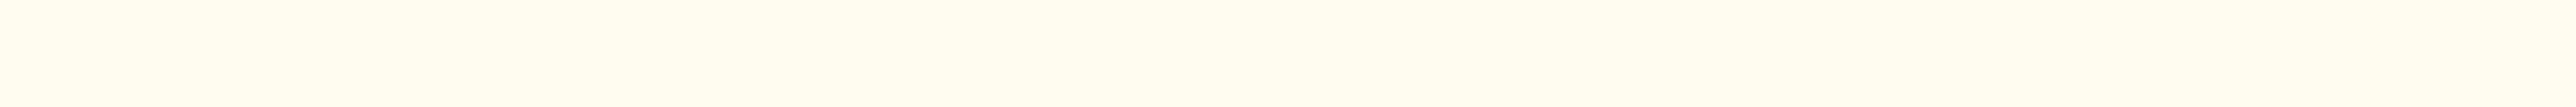
\includegraphics[width=0.2\textwidth]{figures/dummy.pdf}
    \else
        \input{#1}
    \fi
} % 快速编译模式

% 章节标题设置
\ctexset{
  secnumdepth = 3,
  chapter = {
    format = \zihao{-2}\bfseries\centering,
    number = \chinese{chapter},
    name = {第,章}},
  section = {
    format = \zihao{-3}\bfseries},
  subsection = {
    format = \zihao{4}\bfseries}}

% 段落不加入编号
\renewcommand{\paragraph}[1]{
  \par\vspace{0.5\baselineskip}\noindent{\bfseries #1}\quad}

\newenvironment{myproof}[1][\textbf{证明}]{\par\noindent{\heiti #1的证明}\quad}{\hfill$\square$\par\vspace{0.5\baselineskip}}